\documentclass{article}
\usepackage[utf8]{inputenc}
\usepackage{amsmath}
\usepackage{amsfonts}
\usepackage{setspace}

\title{Mathematical Analysis \\ Lecture }
\author{Philip Policki}
\date{12th October 2020}

\usepackage{natbib}
\usepackage{graphicx}
\graphicspath{{./imgs/}}

\begin{document}
\setstretch{1.2}
\maketitle
\tableofcontents
\pagebreak
\section{Rules}
	No textbook, so take notes. \\
	Classes are mandatory
	
\section{Requirements}
	During the classes we will start with a quiz, every practice.
	To pass the course you need $50\%$ of points from the quizzed. A Quizes is 15min every quiz is worth 5 points. You get points from your top 10 quizes.
\section{Notation}
\subsection{Number sets}
\begin{enumerate}
	\item Natural Numbers $ N = \{1, 2, 3, ...\}$ 
	\item Integers $ \mathbb{Z} = \{..., -2, -1, 0, 1, 2, ...\}$
	\item Rational $ \mathbb{Q} = \{ \frac{p}{q}; p, q \in Z, q\neq0 \} $
	\item Irrational $ ex.: \sqrt{2}, \pi, ... $ 
	\item Real Numbers $\mathbb{R} = Rational + Irrational $
\end{enumerate}

\subsection{Sets notation}
$(a, b) = x \in R: a<x<b$ \\
$(a, b) = x \in R: a \leq x \leq b$ \\	
$(a, \infty) = x\in R: x > a$ \\ \\
$(a, b) - open interval$ \\
$ [a, b] - closed interval $ \\ \\
$ A \subset B$ A is a subset of B \\
$ x\in A$ X is an element of A, x belongs to A \\
$ x\notin A$ X is not an element of A, x does not belong to A \\

\subsection{Cartesian Product}
Given two sets A and B, we can form the set consisting of all ordered pairs of the form $(a, b)$ where $a \in A$ and $b \in B$. This set is called the Cartesian product of A and B and is denoted by $AxB$\\
$AxB \{(a, b): a\in A, \in B \}$ \\
If $A=B$, then $AxA$ is denoted by $A^2$\\

\subsection{Quantifiers}
\begin{enumerate}
	\item  Existential $\exists$ "There exists x such that", "For at least one x"
	\item Universal $\forall$ "For all x", "For each x", "For every x"
\end{enumerate}

Example: \\
$ \exists \; t > 0 \; \forall \; x\in \mathbb{R} \; x^2 + 4x + 4 > t $ \\
The statement above is false \\
The negation of the statement: \\
$ \forall \; t>0 \; \exists \; x_0 \in \mathbb{R} \; x_0^2 + 4x_0 + 4 \leq t $

\section{Functions}
A function f is a rule that assigns to each element x in a set A \underline{exactly one} element , called f(x), in a set B. \\
In our class $ A \subset \mathbb{R} $ and $ B \subset \mathbb{R}$
The set A is called the domain of the function f and will be denoted $D_f$.\\
The range of the function f is the set of all possible values of f(x) as x varies throughout the domain. The range of f will be denoted by $R_f$.\\
The most common method for visualizing a function is its.\\ 
If f is a function with domain $D_f$ then its graph is the set of ordered pairs. \\
$ \{(x, y) \in \mathbb{R}^2 \; x\in D_f, y=f(x) \}$ \\ \\
Example: \\ 
Min function  \\
\begin{equation}
	\begin{gathered}
		f(x) = min\{x, x^2\} \\
		f(2) = min\{2, 4\} = 2 \\
		f(\frac{1}{2}) = min\{\frac{1}{2}, \frac{1}{4}\} = \frac{1}{4} \\ \\ \\
	\end{gathered}
\end{equation}

Absolute \\
\begin{equation}
	\begin{gathered}
		f(x) = |x| = \{x, if x \geq 0 \; or -x, if x-2 < 0\}\\
		f(x) = |x -2| = \{x-2, if x \geq 0 \; or -(x-2), if x-2 < 0\} \\ \\
	\end{gathered}
\end{equation}

$|x-a|$ represents the distance between x and a
\subsection{The Vertical Line Test}
A curve is the XY plane is the graph of a function of x if and only if no vertical line intersects the curve more than once.
\subsection{Classes of functions}
\begin{enumerate}
	\item Periodic functions \\
	We say that f is a periodic function if \\ 
	$\exists T>0 \; \forall x\in D_f(x \pm T \in D_f$ and $f(x+T) = f(x))$ \\
	A periodic function is a function that repeats its values after some determined period has been added to its independent variable.\\
	\item Symmetric functions
	\begin{itemize}
		\item Even\\
		A function f is called even if: \\
		$\forall x \in D_f \; (-x  \in D_f)$ and $f(-x) = f(x)$ \\
		The geometric  significance of an even function is that its graph is symmetric with respect to the Y axis. \\
		If f is even $D_f$ is symmetric about the Y Axis.
		\item Odd \\ 
		A function f is called odd if: \\
		$ \forall x \in D_f (-x \in D_f) $ and $f(-x) = -f(x)$\\
		The graph of and odd function is symmetric about the origin.\\
		If an odd function is defined at x=0 then f(0) must be 0!!\\ \\
		Example:
		Check if function is even or odd.\\
		$f(x) = \frac{3^x - 3^{-x}}{x}$
		\begin{enumerate}
			\item Check if domain is symmetric \\
			$D_f = \mathbb{R}\setminus \{0\}$
			\item Substitute -x for x
		\end{enumerate}
	\item Monotonicity: \\
	A function is monotonic if it is increasing, or decreasing, or non-decreasing, or non-increasing.
	\begin{itemize}
		\item Increasing:\\
		A function f is called increasing on a set $I \subset D_f$, \\
		if $\forall x_1, x_2 \in I \; [(x_1 < x_2) \Rightarrow (f(x_1) < f(x_2))]$
		\item Non-decreasing: \\
		A function f is called increasing on a set $I \subset D_f$, \\
		if $\forall x_1, x_2 \in I \; [(x_1 < x_2) \Rightarrow (f(x_1) \leq f(x_2))]$
		\item Decreasing: \\
		A function f is called increasing on a set $I \subset D_f$, \\
		if $\forall x_1, x_2 \in I \; [(x_1 < x_2) \Rightarrow (f(x_1) > f(x_2))]$
		\item Non-increasing: \\
		A function f is called increasing on a set $I \subset D_f$, \\
		if $\forall x_1, x_2 \in I \; [(x_1 < x_2) \Rightarrow (f(x_1) \geq f(x_2))]$
	\end{itemize}
	Algebraic way to check monotonicity: \\
	let $f(x) = \frac{1}{1+x^2}$ and $I = (-\infty, 0]$ \\
	Take any 2 points $x_1, x_2 \in I$ with $x_1 < x_2$. \\
	$f(x_2) - f(x_1) = \frac{1}{1+x_2^2} - \frac{1}{1+x_1^2}$ = \\
	$\frac{1+x_1^2 - 1 + x_2^2}{(1+x_1^2)(1+x_2^2)}$ = \\
	$\frac{(x_1-x_2)(x_1+x_2)}{(1+x_2^2)(1+x_1^2)}$ \\
	$x_1 - x_2  < 0$ \\
	$x_1 + x_2 < 0$ \\
	\end{itemize}
	\end{enumerate}
	\subsection{New functions from Old functions}
	\begin{itemize}
		\item Vertical and horizontal shifts: \\
		Suppose $c>0$.\\ To obtain the graph of $y = f(x) + c$ shift the graph of y a distance of c units upwards. If $y = f(x)-c$ shift downwards. \\ \\
		To obtain the graph of $y=f(x-c)$ shift the graph y a distance of c units to the right. \\
		To obtain the graph of $y=f(x+c)$ shift the graph y a distance of c units to the left. \\
		\item Vertical and horizontal stretching and reflecting: \\
		Suppose $c>1$. \\
		To obtain the graph $y=c*f(x)$ stretch y vertically by a factor of x. \\
		To obtain the graph $y=f(c*x)$ compress the graph of y horizontally by a factor of c. \\
		To obtain the graph $y=-f(x)$ reflect the graph of y about the y axis. \\
		To obtain the graph $y=f(-x)$ reflect the graph of y about the x axis. \\
		\item Algebra of functions: \\
		let f and g be functions with domains $D_f$ and $D_g$. Then the functions $f_g$, $f-g$, $fg$ and $\frac{f}{g}$ are as follows: \\
		$(f\pm g)(x) = f(x)\pm g(x)$; $D_{f+g} = D_f \cap D_g$ \\ 
		$(f* g)(x) = f(x)*g(x)$; $D_{f*g} = D_f \cap D_g$\\
		$(\frac{f}{g})(x) = \frac{f(x)}{f(g)}$; $D_{f+g} = D_f \cap D_g$
	\end{itemize}
	\subsection{Composite Functions}
	Given 2 functions f and g the \underline{composite} function is denoted by $f \circ  g$ and is defined as $(f \circ g)(x) = f(g(x)))$.\\
	
	\underline{Example:} \\
	If $f(x) = \sqrt{2-x}$ and $g(x) = \sqrt{x}$, then: \\
	$(f \circ g)(x) = f(g(x)) = \sqrt{2-\sqrt{x}}$ \\
	$(g \circ f)(x) = g(f(x)) = \sqrt{\sqrt{2-x}}$  \\
	For a $\sqrt{x}$ to be defined, we must have $x\geq 0$. For $\sqrt{2-\sqrt{x}}$ to be defined we must have a $2-\sqrt{x} \geq 0$ that is $\sqrt{x} \leq 2$ or $x\leq 4$. One can see that $D_{f\circ g} = [0, 4]$ therefore $D_{g\circ f} = (-\infty, 2]$ \\ \\
	Let $h(x) = 3^{\sqrt{x+3}}$, write it as $f \circ g$: \\
	$f(x) = 3^x$ \\ $g(x) = \sqrt{x+3}$ \\
	$(f^{-1} \circ f)(x) = x, \forall x\in D_f$ \\
	$(f \circ f^{-1})(x) = x, \forall x\in R_f$
	\subsection{One-to-one functions}
	A function f is called an one-to-one function on a set $I \subset D_f$ \\
	$\forall x_1, x_2 \in I$ $[(x_1 \neq x_2) \Rightarrow (f(x_1) \neq f(x_2))]$ \\
	\underline{Example:}
	\begin{itemize}
		\item (Strictly) increasing function are 1-1
		\item Exponential functions are 1-1
	\end{itemize}
	\subsubsection{Horizontal Line Test}
	A function f in one-to-one if and only if no horizontal line intersects the graph at most once \\ \\
	
	Let f be a 1-1 function with a domain $D_f$ and a range $R_f$. Then its \underline{inverse function} $f^{-1}$ has a domain $D_{f^{-1}} = R_f$ and $R_{f^{-1}} = D_f$ and is defined by: \\
	$(f^{-1})(y) = x \Leftrightarrow f(x) = y$ \\
	\underline{Example:}\\
	Let $g(x) = 3+x+2^x$. Is g invertible ? Yes, because its a strictly increasing function.\\
	The inverse of $y=a^x$ is $y=\log_ax$ where $a>1$. \\
	The inverse of $y=a^x$ is $y=\log_ax$ where $0<a< 1$.\\ 
	\pagebreak
	\section{Logarithms}
	The logarithm to the bare a is defined as the inverse function of the exponential function with bare a, that is $y=\log_ax$ means that $x=a^y$
	
	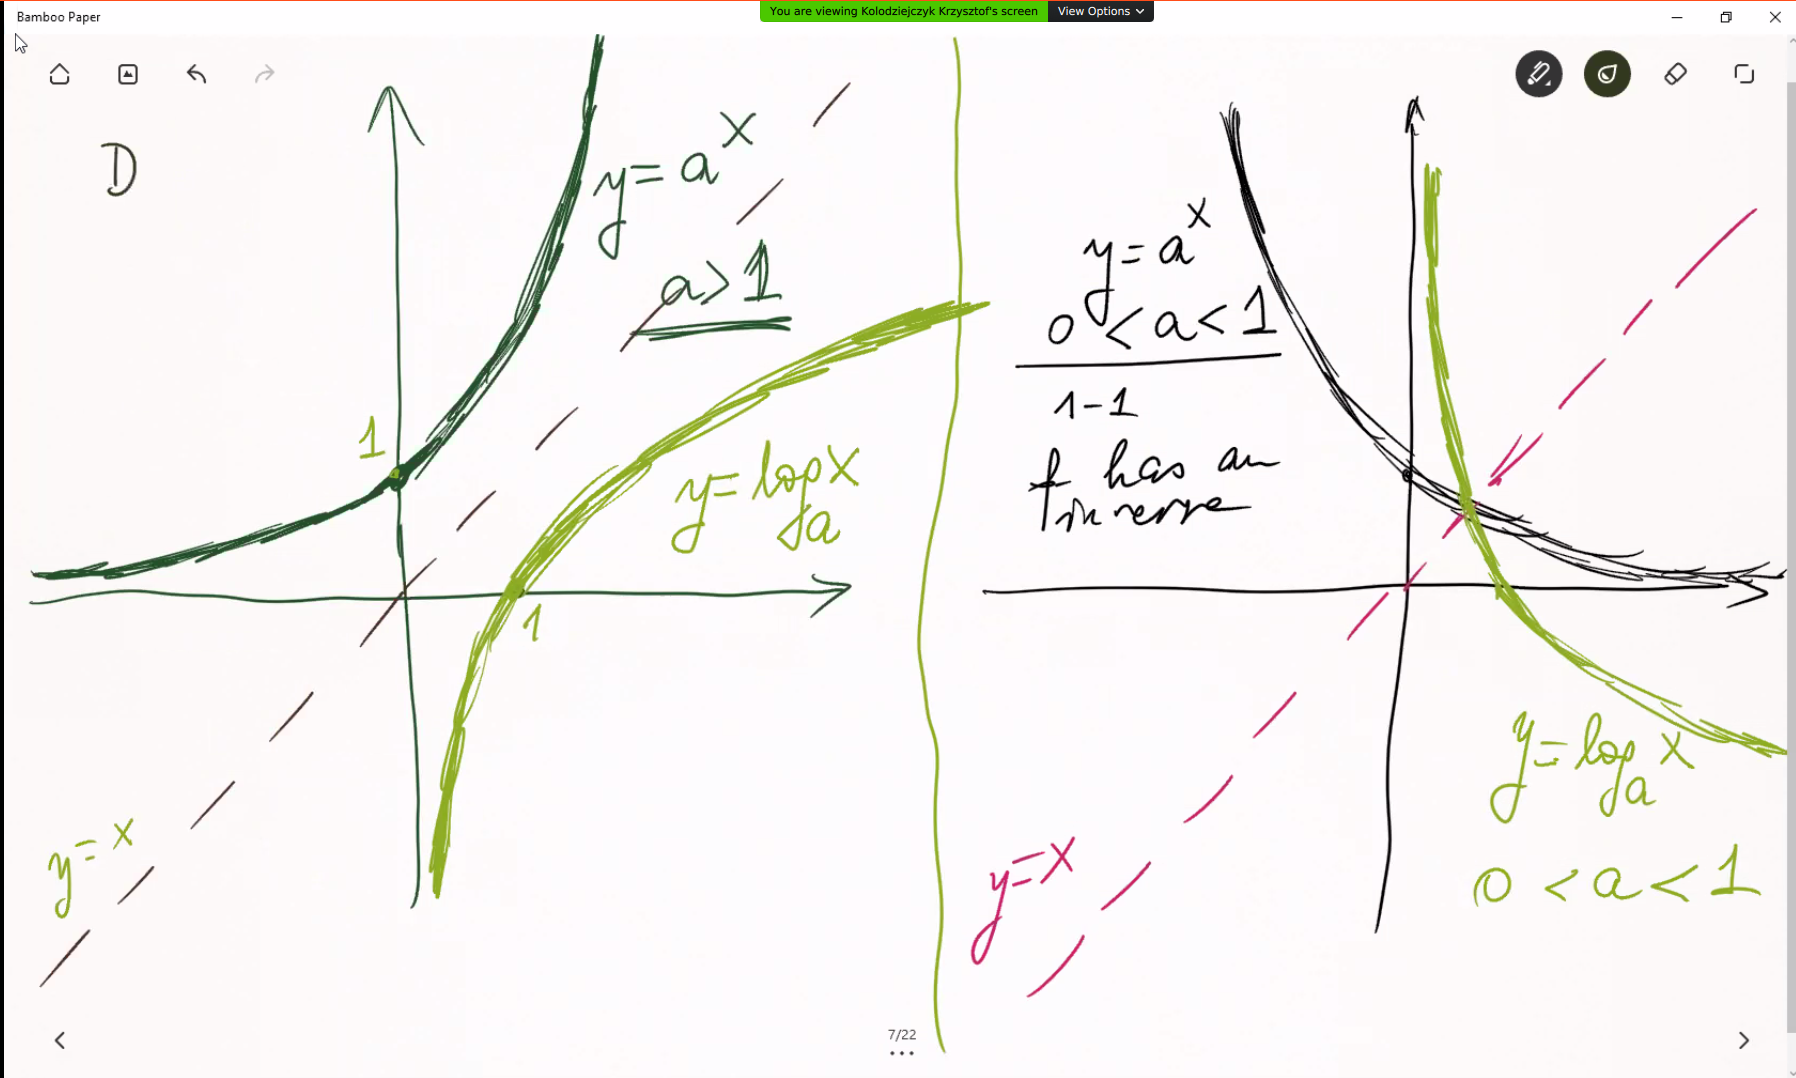
\includegraphics[scale=0.17]{1.png}
	
	\subsection{Laws of logarithms}
	\begin{enumerate}
		\item $\log_a(bc) = \log_ab + \log_ac$
		\item $\log_ab^c = c*\log_ab$
		\item $\log_a\frac{b}{c} = \log_ab - \log_ac$
		\item $\log_ac = \log_ab * \log_bc$
	\end{enumerate}
	\pagebreak
	\section{Trigonometry}
	A standard position of an angle occurs when we place its vertex at the origin of a coordinate system and initial side on the positive x-axis. \\
	A positive angle is obtained by rotating the initial side counterclockwise until it coincides with the terminal side. Negative angles are obtained by a clockwise rotation. Angles can be measured in radians. Mandatory for this class. \\
	For an acute angle $\alpha$ the trigonometric functions are defined as ratios. \\
	$\sin(\alpha) = \frac{opposite}{hypothenuse}$ \\
	$\cos(\alpha) = \frac{adjacent}{hypothenuse}$ \\
	$\tan(\alpha) = \frac{opposite}{adjacent}$ \\
	$\cot(\alpha) = \frac{adjacent}{opposite}$ \\
	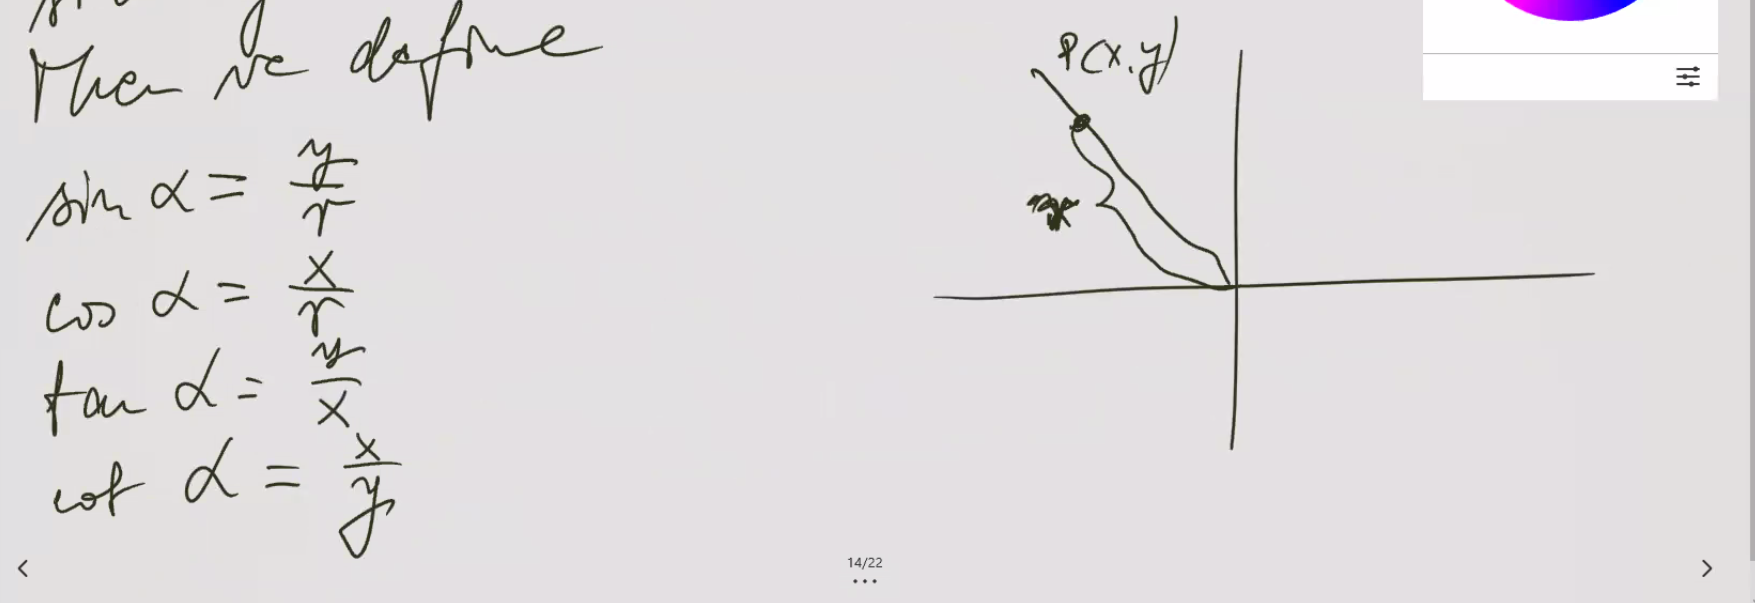
\includegraphics[scale=0.2]{2.png} 
	The signs of the trig functions for angles in each of the quadrants can be remembered with: "\textbf{A}ll \textbf{S}tudents \textbf{T}ake \textbf{C}alculus"
	\pagebreak
	\subsection{Trigonometric identities}
	We have a angle $\alpha$ and a point $P(x, y)$\\
	
	\begin{itemize}
		\item $\forall \alpha \in \mathbb{R}$  $\sin^2\alpha + \cos^2\alpha = 1$
		\item $\forall \alpha \in \mathbb{R}$  $\sin(-\alpha) = -\sin\alpha$
		\item $\forall \alpha \in \mathbb{R}$  $cos(-\alpha) = \cos\alpha$
		\item $\forall \alpha \in \mathbb{R}$  $\sin(\alpha + 2\pi) = \sin(\alpha)$ and $\cos(\alpha + 2\pi) = \cos(\alpha)$
		\item $\sin(x+y) = \sin(x)\cos(y)  + \cos(y)\sin(x)$
		\item $\sin(x-y) = \sin(x)\cos(y)  - \cos(y)\sin(x)$
		\item $\sin(2x) = 2\sin(x)\cos(x)$
		\item If we denote $x+y=\alpha$ and $x-y=\beta$, then \\ $\sin(\alpha) + \sin(\beta) = 2\sin(\frac{\alpha + \beta}{2})*\cos(\frac{\alpha - \beta}{2})$
		\item $\cos(x+y) = \cos(x)\cos(y) - \sin(x)\sin(y)$
		\item $\cos(x-y) = \cos(x)\cos(y) + \sin(x)\sin(y)$
		\item $\cos(\alpha) + \cos(\beta) = 2\cos(\frac{\alpha + \beta}{2})*\cos(\frac{\alpha - \beta}{2})$
		\item $\cos(2x) = \cos^2(x) - \sin^2(x)$
		\item $\cos^2(x) = \frac{1 + \cos(2x)}{2}$
	\end{itemize}
	\pagebreak
	\subsection{Reduction formulas}
	\begin{itemize}
		\item $\sin(\alpha + k\frac{\pi}{2}) = \sin(\alpha)\cos(k\frac{pi}{2}) + \cos(\alpha)\sin(k\frac{\pi}{2})$
		\subitem when k is even $\pm \sin(\alpha)$
		\subitem when k is odd $\pm \cos(\alpha)$
		\item $\cos(\alpha + l\frac{\pi}{2})=\cos(\alpha)\cos(k\frac{\pi}{2}) - \sin(\alpha)\sin(k\frac{\pi}{2})$
		\subitem when k is even $\cos(\alpha)$
		\subitem when k is odd  $\pm\sin(\alpha)$
	\end{itemize}
	\subsection{Inverse of trigonometric functions / Cyclometric functions}
	The function $\sin(x)$ is not 1-1 but if we consider $f(x) = \sin(x)$ for $x\in [\frac{-\pi}{2}, \frac{\pi}{2}]$ as a 1-1 function The existing inverse is called arcsine $\arcsin(x)=y \Leftrightarrow \sin(y)=x$ and $\frac{-\pi}{2} \leq \frac{\pi}{2}$
	\begin{center}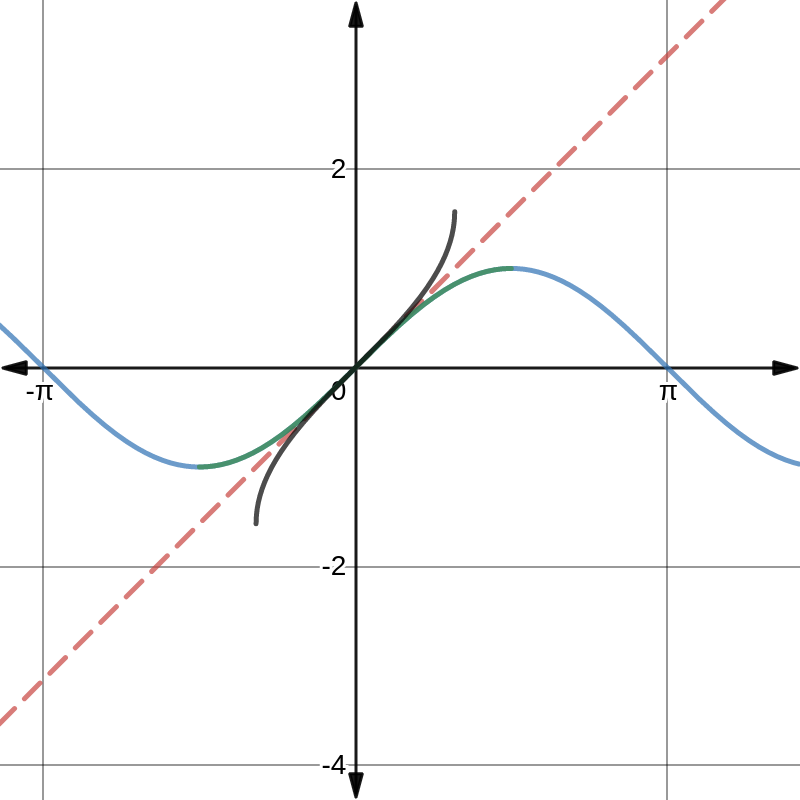
\includegraphics[scale=0.25]{4.png}\end{center}
	The function $\cos(x)$ is not 1-1 but if we consider $f(x) = \cos(x)$ for $x\in [0, \pi]$ as a 1-1 function The existing inverse is called arc-cosine $\arccos(x)=y \Leftrightarrow \sin(y)=x$ and $0 \leq \pi$ 
	\begin{center}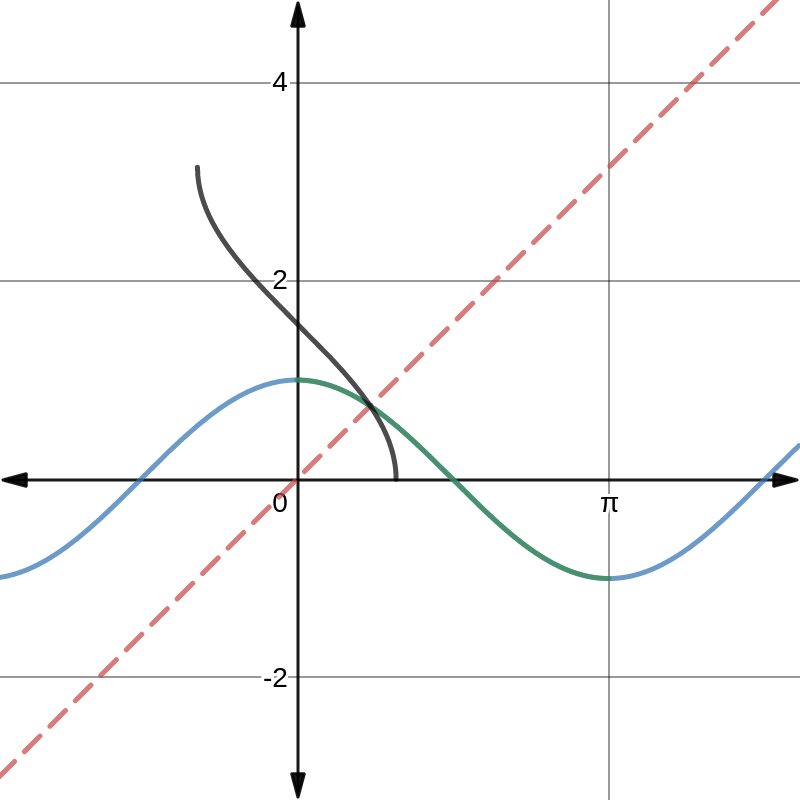
\includegraphics[scale=0.25]{3.png}\end{center}
 	\underline{Example: }\\
 	Show that $\arcsin(x) + \arccos(x) = \frac{\pi}{2}$\\
 	$\arcsin(x) = \alpha \Leftrightarrow \sin(\alpha) = x$ and $\frac{-\pi}{2} \leq \alpha \leq \frac{\pi}{2}$ \\
 	$\arccos(x) = \beta \Leftrightarrow \cos(\beta) = x$ and $0 \leq \beta \leq \pi$ \\
 	\section{Sequences}
 	A sequence can be thought of as a list of numbers written in a definite order ex. $a_1, a_2, ..., a_n$. The numbers have special names\\ $a_1$ is called the first term of the sequence. $(a_n)$ infinite sequence of numbers, $\{a_n\} = \{a_n: n \in\mathbb{N} \}$. \\
 	A sequence can be defined as a function whose domain is is the set $\mathbb{N}$. But we usually write $a_n$ instead of the function notation f(n).\\
 	Sequences can be defined by: 
 	\begin{enumerate}
 		\item By giving the formula for the nth term: $a_n = \frac{(-1)^{n+1}(n+\sqrt[n]{n})}{2^n}$
 		\item By a description: Let $a_n$ be the digit in the n-th decimal place of the number $\sqrt{2}$
 		\item By a recursive relation: $f_1 = 1, f_2 = 1, f_n = f_{n-1} + f_{n-2}\; \forall \; n \geq 3$
 	\end{enumerate}
 \pagebreak
 	\subsection{Limit Laws for convergent sequences}
 	If $(a_n)$ and $(b_n)$ are convergent sequences and c is a constant then:
 	\begin{enumerate}
 		\item $\lim_{n \to \infty } (a_n+b_n) = \lim_{n\to\infty} a_n + \lim_{n\to\infty} b_n$
 		\item $\lim_{n \to \infty } (c*a_n) = c\lim_{n \to \infty } (a_n)$
 		\item $\lim_{n \to \infty } (a_n*b_n) = \lim_{n \to \infty } (a_n) * \lim_{n \to \infty } (b_n)$
 		\item $\lim_{n \to \infty } (\frac{a_n}{b_n}) = \frac{\lim_{n \to \infty } (a_n)}{\lim_{n \to \infty } (b_n)}$ if $\lim_{n \to \infty } (b_n) \neq 0$ 
 		\item $\lim_{n \to \infty } (a_n)^p = (\lim_{n \to \infty }a_n)^p$
 		\item $\lim_{n \to \infty } (\sqrt[n]{a_n}) = \sqrt[k]{\lim_{n \to \infty } (a_n)}$
 		\item $\lim_{n \to \infty } (\sqrt[n]{a}) = 1$
 		\item $\lim_{n \to \infty } (\sqrt[n]{n}) = 1$
 	\end{enumerate}
 	\subsubsection{Squeeze Theorem for sequences}
 	If $a_n \leq b_n \leq c_n$ for $n \geq n_0$.\\
 	and \\
 	$\lim_{n\to\infty} a_n = \lim_{n\to\infty} c_n = L$, then $\lim_{n\to\infty} b_n = L$ \\ \\
 	A sequence is bounded above if there is a number such that $a_n \leq M $
 
 
 
 
 
 
 
 
 
 
 
 
 
 
 
 
 
 
 
 
 
 
 
 
 
 
 
 
 
\end{document}